%%%%%%%%%%%%%%%%%%%%%%%%%%%%%%%%%%%%%%%%%%%%%%%%%%%%%%%%%%
% # Elicited Production Experiment
%%%%%%%%%%%%%%%%%%%%%%%%%%%%%%%%%%%%%%%%%%%%%%%%%%%%%%%%%%

\chapter{Elicited Production Experiment}\label{ch-ept}

% \excnt=108

This chapter reports on the elicited production task (EPT) I used in the ORC and SRC studies to test whether resumption facilitates production of RCs under processing strain. I begin in Section \ref{ept-rq} by listing the research questions (RQs) that guided the creation of this task. I~describe the design of the task in Section \ref{ept-design} and the data analysis procedures in Section \ref{ept-analysis}. In Sections \ref{ept-result-token}--\ref{ept-result-proficiency}, I walk the reader through the results, addressing each of the RQs in turn. Section \ref{ept-conclusion} concludes the chapter.

%========================================================%
\section{Research questions}\label{ept-rq}
%========================================================%

I had three main RQs for the EPT, all of which pertain to the production of resumptive RCs in L1 and/or L2 English:\vspace{5pt}

\begin{enumerate}[\bfseries RQ1:,itemsep=5pt]
\item {\bfseries How does processing strain affect rates of resumption?}\par\nobreak
Prediction: Participants will produce resumptive RCs more often in environments that are relatively difficult for relativization than in environments that are relatively easy for relativization. This would suggest that resumption facilitates RC production when there is strain on the processor.
\end{enumerate}\vspace{5pt}

\begin{enumerate}[\bfseries RQ2:,itemsep=5pt]
\item {\bfseries Which form of resumption is dominant?}\par\nobreak
Prediction: Participants will produce more tokens of RP resumption than tokens of full-NP resumption, in line with general pragmatic requirements for referring expressions in English (see~Section~\ref{pro-aboutness}).
\end{enumerate}\vspace{5pt}

\begin{enumerate}[\bfseries RQ3:,itemsep=5pt]
\item {\bfseries How does L2 proficiency affect rates of resumption?}\par\nobreak
Prediction: Higher-proficiency L2ers will produce resumptive RCs less often than lower-proficiency ones, at least in environments where English allows gapping. Such a pattern of results would suggest that (a)~processing efficiency increases over the course of L2 acquisition and/or (b)~L2ers become more sensitive to the English prohibition on RC resumption as their level of proficiency rises.
\end{enumerate}

%========================================================%
\section{Design and procedure}\label{ept-design}
%========================================================%

The task had 15 critical items (3 conditions × 5 tokens, Latin squared) eliciting RCs from the three levels on the SLW hierarchy---short-distance (henceforth, the Short condition), long-distance (henceforth, the Long condition), and \textit{wh}-island (henceforth, the Island condition)---the assumption being that these are increasingly difficult relativization environments. Tables \ref{tab:ept-cond-orc} and \ref{tab:ept-cond-src} show examples of target responses in the three critical conditions for the ORC and SRC versions of the EPT.

\begin{table}
\caption{Critical conditions in the ORC elicited production task}\label{tab:ept-cond-orc}
\raggedright\setstretch{1}
\begin{tabularx}{\linewidth}{lX}\toprule
Environment~~ & Target Response \\\midrule
Short & the man that the officers arrested \{\_\_/*him\} last week \\
Long & the man that Mary thinks the officers arrested \{\_\_/*him\} last week \\
Island & the man that Mary wonders which officers arrested \{*\_\_/*him\} last week \\\bottomrule
\end{tabularx}
\vspace{-12pt}
\end{table}

\begin{table}
\caption{Critical conditions in the SRC elicited production task}\label{tab:ept-cond-src}
\raggedright\setstretch{1}
\begin{tabularx}{\linewidth}{lX}\toprule
Environment~~ & Target Response \\\midrule
Short & the man that \{\_\_/*he\} borrowed a book last month \\
Long & the man that Mary thinks \{\_\_/*he\} borrowed a book last month \\
Island & the man that Mary wonders which book \{*\_\_/*he\} borrowed last month \\\bottomrule
\end{tabularx}
\vspace{-12pt}
\end{table}

\noindent There were also 15 fillers, all eliciting short-distance SRCs from biclausal sentences. Target responses for three of these fillers are shown in (\ref{ex-ept-fill}). The full list of critical and filler stimuli can be found in Appendix \ref{app-materials-ept}.

\pex\label{ex-ept-fill}
\a the woman that wonders which criminals attacked John last night
\a the man that says Tina baked a cake last night
\a the woman that says the firefighters saved Dave last week
\xe 

As explained in Section \ref{stu-slw}, I expected that the Short-condition trials would be easy to process for ENSs and L2ers alike. The Long-condition trials, which, recall, were much simpler than long-distance trials in L1 adult English studies such as the one by Hofmeister and Norcliffe (\citeyear{hofmeister.norcliffe2013}), were designed to be easy for ENSs but potentially challenging for L2ers (see~Section~\ref{stu-slw}). Finally, I~anticipated that the Island-condition trials would impose a considerable processing burden on participants in all three groups due to the high cost associated with extending an RC dependency into a \textit{wh}-clause (see~Section~\ref{gap-lw}), especially with such RCs being (a)~ill-formed in English and (b)~rarely encountered in the English input. I reasoned that if resumption eases RC production under processing strain, then rates of responses containing resumptive RCs should increase across conditions from Short (easiest) to Island (hardest).

RCs were elicited following a procedure loosely modeled on the one used by \textcite{ferreira.swets2005}. Each trial consisted of two panels presented sequentially on a computer screen, as illustrated in Figures \ref{fig:ept-trial-orc} and \ref{fig:ept-trial-src}, which are critical items in the Island condition from the ORC and SRC studies.

\begin{figure}
\caption{Island-condition trial in the ORC elicited production task} \label{fig:ept-trial-orc}
\raggedright\setstretch{1}
\begin{tabularx}{\linewidth}{|X|X|}\hline

\includegraphics[width=3.15in]{../image/ept-trial-orc-a.png} & 
\includegraphics[width=3.15in]{../image/ept-trial-orc-b.png} \\\hline
\end{tabularx}
\textit{Note}. Participants first saw the panel on the left and then the panel on the right.
\vspace{-12pt}
\end{figure}

\begin{figure}
\caption{Island-condition trial in the SRC elicited production task} \label{fig:ept-trial-src}
\raggedright\setstretch{1}
\begin{tabularx}{\linewidth}{|X|X|}\hline

\includegraphics[width=3.15in]{../image/ept-trial-src-a.png} & 
\includegraphics[width=3.15in]{../image/ept-trial-src-b.png} \\\hline
\end{tabularx}
\textit{Note}. Participants first saw the panel on the left and then the panel on the right.
\vspace{-12pt}
\end{figure}

\noindent The first panel had pictures of two similar-looking men/women accompanied by descriptive sentences: One of these was the test sentence and the other was a foil which differed from the test sentence by only one word and which was included to create a felicitous context for relativization (\cite{ferreira.swets2005}, p.~269; \cite{goodluck.stojanovic1996}, p.~297; \cite{hamburger.crain1982}; \cite{kim2013}, p.~18ff; \cite{kim.ogrady2019}, p.~8; \cite{labelle1990}, p.~97). The position of the test sentence (top or bottom) was counterbalanced across trials.

The second panel was identical to the first except that the test sentence was replaced by a question (`Which man/woman is this?'). The `Recording...' message at the bottom of this panel notified participants that their voices were being recorded. Starting from when the second panel appeared on the screen, participants had six seconds in which to give their full response, and afterwards they had the option to listen to their response and/or record it again before moving to the next trial. Only the final recording was retained for analysis. Participants could re-record their responses as many times as they wished (in case they were not able to complete their response in the time allotted when they were becoming familiar with the procedure), but they were not permitted to return to the first panel with the test sentence.

Participants read the instructions and completed three practice trials before starting the main phase of the task. For the practice trials, they had to select an appropriate response in multiple-choice format instead of producing an oral response. The purpose of the practice phase was to familiarize participants with the procedure and to increase the likelihood that they would produce RCs during the main portion of the task. During the practice phase, participants were notified when their answers were incorrect (in their native language, to ensure comprehension), and those with one or more incorrect responses were made to repeat the instructions and practice questions until they answered all three items correctly. Participants received the same three practice items every time they entered the practice phase of the task, but the presentation order was randomized each time.

%========================================================%
\section{Data processing and analysis}\label{ept-analysis}
%========================================================%

Responses were transcribed and categorized by two coders. The response categories were as follows: `Gapping' (a gapped RC of the target type), `Resumption' (a resumptive RC of the target type), `Other' (any other gapped or resumptive RC containing relevant information), and `Nontarget' (any response lacking an RC or failing to reference information in the sentences). Lexical errors (e.g.,~using names from the foil sentences rather than those from the test sentences) were ignored. Example responses in each category for the items in Figures \ref{fig:ept-trial-orc} and \ref{fig:ept-trial-src} are provided in (\ref{ex-ept-sample-orc}) and (\ref{ex-ept-sample-src}), respectively. 

\pex Example Island-condition responses in each category in the ORC elicited production task \label{ex-ept-sample-orc}\par\nobreak
\a Gapping: \par\nobreak\vspace{5pt}
the man Mary wonders which officers arrested last week (ENS\_ORC\_10) \par\nobreak
the one that Mary wonders which officers arrested last week (KLE\_ORC\_12) \par\nobreak
this man that Mary wonders which officers arrested last week (MLE\_ORC\_48)
\a Resumption: \par\nobreak\vspace{5pt}
the one that Mary wondered which officers had arrested him last week (ENS\_ORC\_29) \par\nobreak 
the one who Mary wonders which officers arrested him last week (KLE\_ORC\_15) \par\nobreak 
He's the one who Mary wonders which officers arrested this man last week (KLE\_ORC\_61) 
\a Other: \par\nobreak\vspace{5pt}
the man that is wondered by Mary which officers arrested last week (KLE\_ORC\_37) \par\nobreak 
the man who Lisa wonder arrested by officer last week (KLE\_ORC\_54) \par\nobreak 
the man Mary wondered who was arrested by which officer last week (MLE\_ORC\_34)
\a Nontarget: \par\nobreak\vspace{5pt}
Mary wonders which officers arrest this man last week (KLE\_ORC\_53) \par\nobreak 
Mary wonders that officers arrested this man last week (KLE\_ORC\_55) \par\nobreak 
This woman wonders that which officers arrested the man last week (MLE\_ORC\_45)
\xe 

\pex Example Island-condition responses in each category in the SRC elicited production task \label{ex-ept-sample-src}\par\nobreak
\a Gapping: \par\nobreak\vspace{5pt}
the man who Mary wonders which book borrowed last month (KLE\_SRC\_02) \par\nobreak
the man that Mary wonders which book borrowed last month (KLE\_SRC\_21) \par\nobreak 
the man that Lisa wonders which book borrowed last month (KLE\_SRC\_27)
\a Resumption: \par\nobreak\vspace{5pt}
the man that Mary wondered which book he borrowed last month (ENS\_SRC\_10) \par\nobreak 
the one that Mary wonders which book this man borrow last month (KLE\_SRC\_17) \par\nobreak 
the man that Mary wonders which book he borrowed last month (MLE\_SRC\_22) 
\a Other: \par\nobreak\vspace{5pt}
the man who borrowed a book that Mary wonders about (ENS\_SRC\_34) \par\nobreak 
the man who borrowed a book last month and Mary wanted to know the book's thesis (KLE\_SRC\_35) \par\nobreak 
the man wondered by Mary for which book did he borrowed last month (KLE\_SRC\_37)
\a Nontarget: \par\nobreak\vspace{5pt}
Mary wondered which book this man borrowed last month (ENS\_SRC\_20) \par\nobreak 
Mary wonders which book this man borrowed last month (KLE\_SRC\_11) \par\nobreak 
Mary wonders which book he borrowed last month (MLE\_SRC\_47)
\xe 

\noindent Inter-rater reliability was high, with Cohen's Kappa calculated at $\kappa$~= .89 (ENS:~.91; KLE:~.90, MLE:~.87) for the ORC dataset and $\kappa$~= .89 (ENS:~.96; KLE:~.90; MLE:~.84) for the SRC dataset. Coding differences were resolved through discussion.

Ten participants were excluded from the ORC dataset for giving only Nontarget responses (ENS: 1/90~= 1\%; KLE: 4/69~= 6\%; MLE: 5/76~= 7\%), leaving 89 ENSs, 65 KLEs, and 71 MLEs for the data analyses. In the SRC dataset, one MLE (1/73 = 1\%) was lost due to experimental error, and an additional seven participants were removed for producing only Nontarget responses (ENS: 2/61~= 3\%; KLE: 1/66~= 2\%; MLE: 4/73~= 5\%), leaving 59 ENSs, 65 KLEs, and 68 MLEs.

For statistical analysis, responses were recoded as [\textsc{±resumption}] (Resumption = [\textsc{+resumption}]; Gapping = [\textsc{−resumption}]; Other = [\textsc{−resumption}]; Nontarget = [\textsc{−resumption}]) and fit to a separate mixed-effects logistic regression model for each study. Pairwise comparisons examined the contrasts for \textsc{environment} (Long − Short; Island − Short; Island − Long) for each level of \textsc{group} (ENS; KLE; MLE). If resumption facilitates RC production under processing strain, then Resumption responses should increase in frequency as the syntactic environment becomes more difficult for relativization. Recall that I predicted that the number of Resumption responses would increase across conditions from Short (lowest) to Island (highest) for all groups; such a pattern of results would suggest that processing load drives the production of resumptive RCs in L1 and L2 English.

To test for L2 proficiency effects on the resumption rates, I repeated the mixed-effects model analyses on the L2 data for each study with scaled English proficiency scores (henceforth, \textsc{proficiency}) added as a continuous fixed effect.\footnotemark{} Reasoning that KLEs and MLEs might have less need to resort to resumption as proficiency increases and processing becomes more efficient, I expected that higher-proficiency L2ers would have fewer Resumption responses than lower-proficiency ones, particularly in the Short and Long conditions, where gaps are grammatical in English.

\footnotetext{See Section~\ref{stu-analysis} for the logic behind scaling the proficiency scores prior to modeling; scaling was done separately for the ORC data and the SRC data.}

%========================================================%
\section{Response rates}\label{ept-result-token}
%========================================================%

To address RQ1, which asks how processing strain affects rates of resumption, I examined how the number of Resumption responses varied across conditions. The mean production rates for Gapping responses, Resumption responses, and Other responses in the ORC and SRC datasets are shown in Figures \ref{fig:ept-token-orc} and \ref{fig:ept-token-src}, respectively.

\begin{figure}
\caption{Means of the by-participant response rates in the ORC elicited production task} \label{fig:ept-token-orc}
\raggedright\setstretch{1}
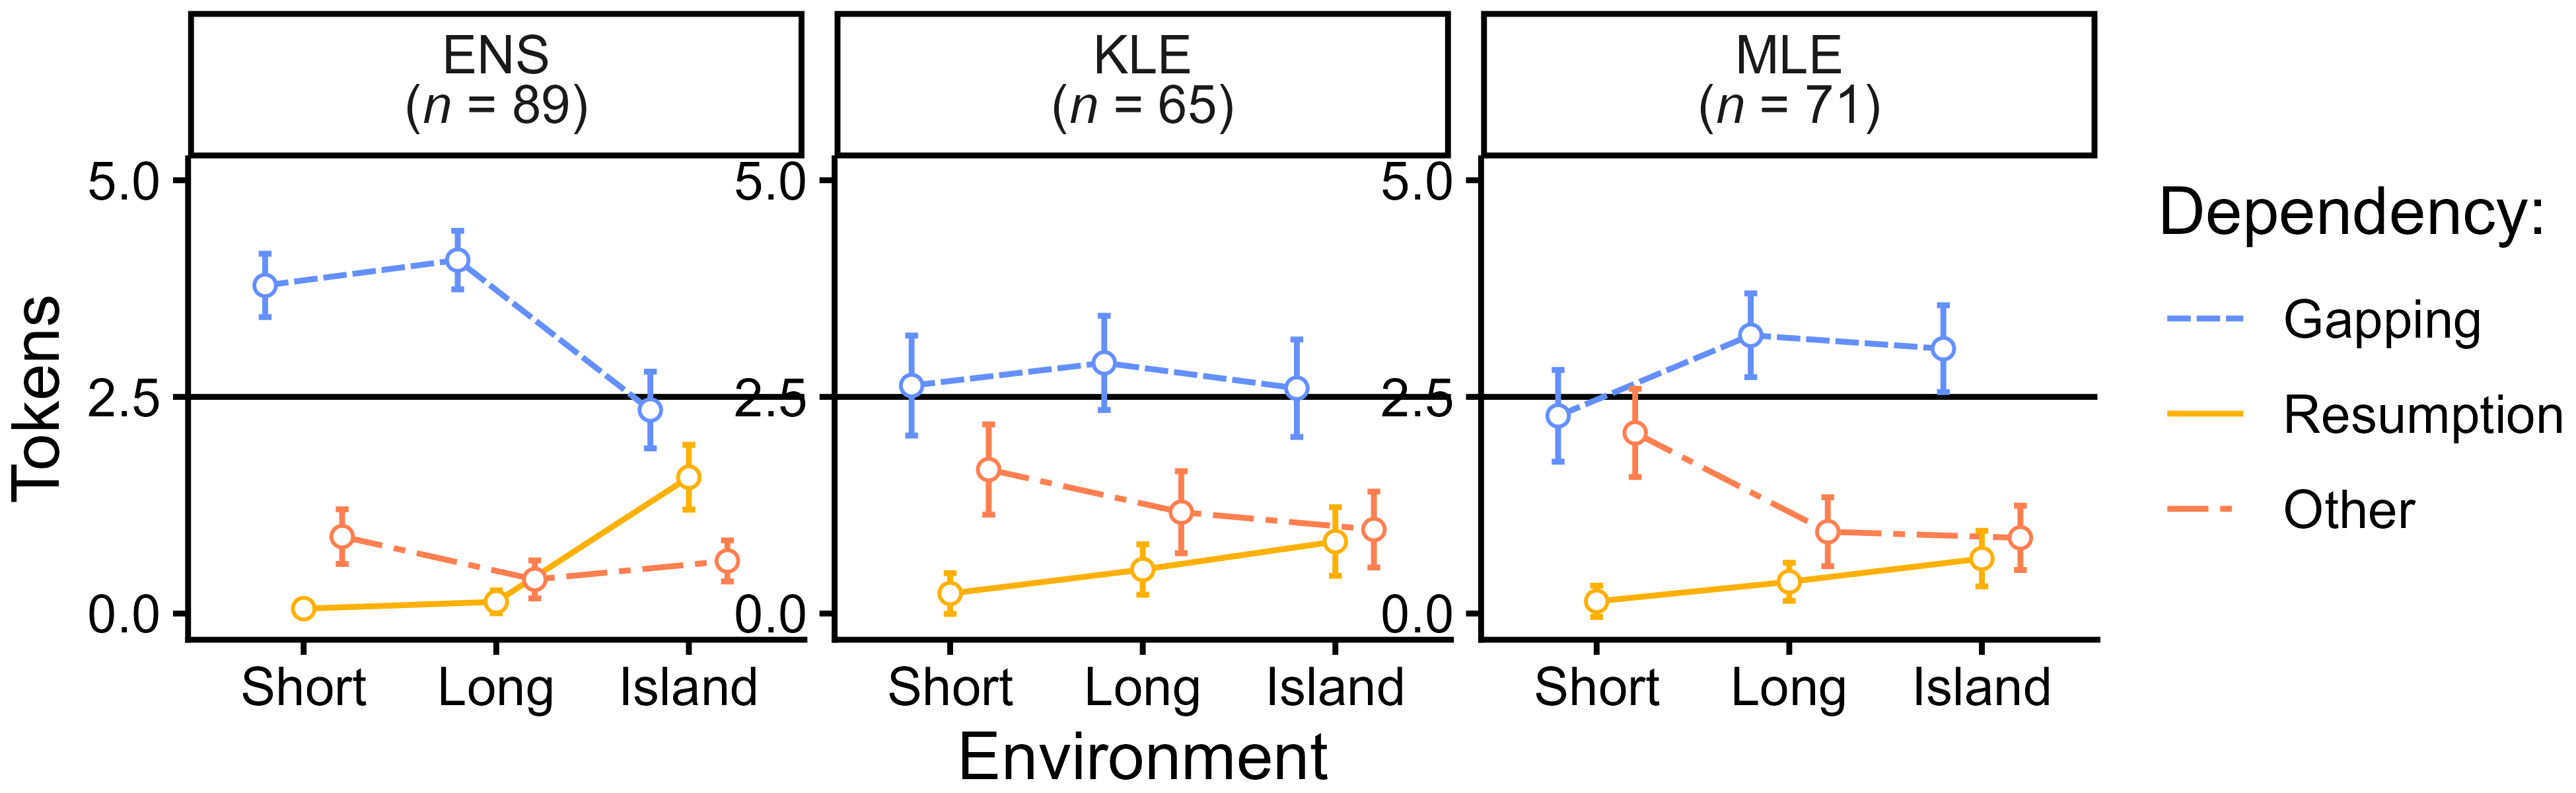
\includegraphics{../analysis/plots/orc_ept_token.png}
\textit{Note}. Max = 5 tokens per condition; error bars are 95\% \textit{CI}s; center line represents 50\% of responses; Nontarget responses are omitted.
\vspace{-12pt}
\end{figure}

\begin{figure}
\caption{Means of the by-participant response rates in the SRC elicited production task} \label{fig:ept-token-src}
\raggedright\setstretch{1}
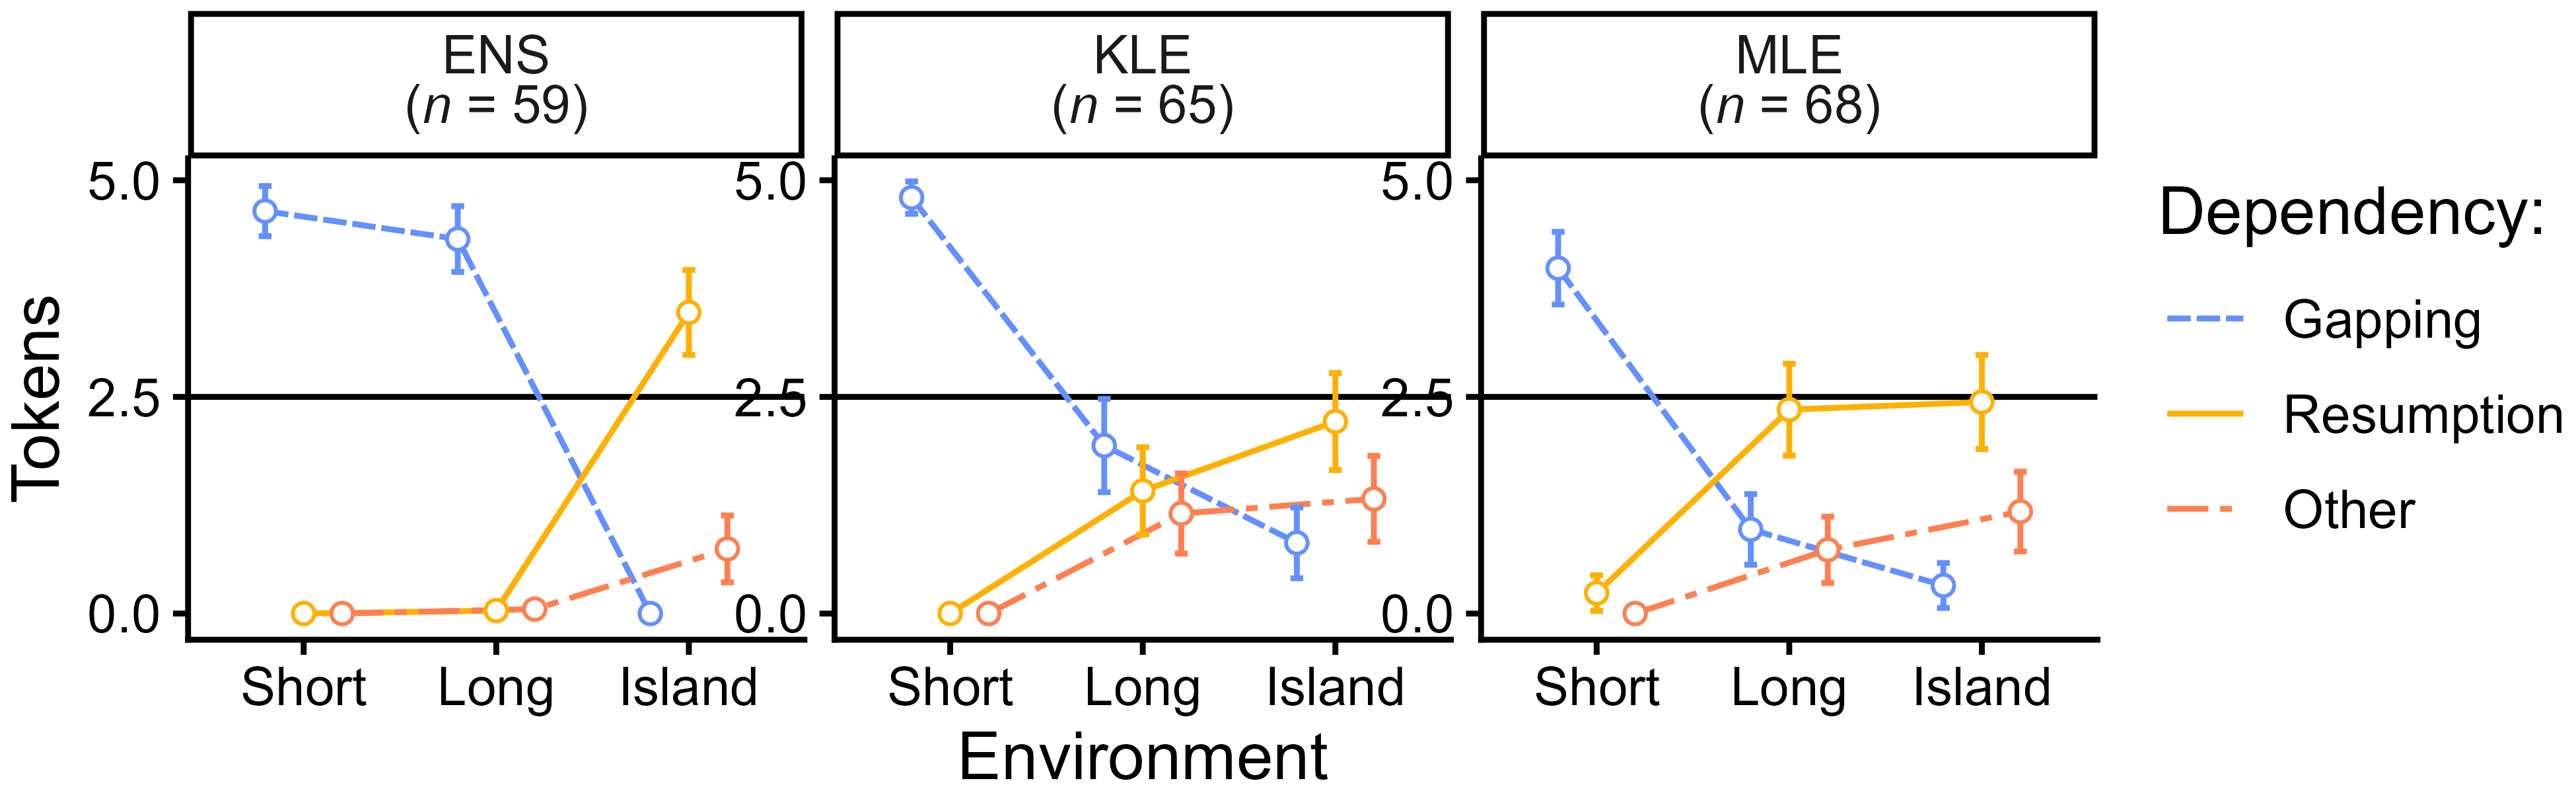
\includegraphics{../analysis/plots/src_ept_token.png}
\textit{Note}. Max = 5 tokens per condition; error bars are 95\% \textit{CI}s; center line represents 50\% of responses; Nontarget responses are omitted.
\vspace{-12pt}
\end{figure}

Rates of Resumption responses increased across conditions for each group from Short (lowest) to Island (highest). In the Island condition, Resumption responses constituted 21\% of all responses in the ORC dataset (ENS:~31\%; KLE:~17\%; MLE:~13\%) and 54\% of all responses in the SRC dataset (ENS:~69\%; KLE:~44\%; MLE:~49\%). By contrast, Resumption responses were least frequent in the Short condition, especially in the SRC dataset, where ENSs and KLEs produced no Resumption tokens whatsoever. The fact that Resumption responses were produced more often in environments thought to be harder for relativization than in environments thought to be easier for relativization suggests that resumption represents a strategy for managing processing overload during RC production.

In the SRC dataset, the rate of Gapping responses tended to decrease across conditions from Short (highest) to Island (lowest). This is exactly the pattern we would expect if the difficulty of producing gapped RCs increases across levels of the SLW hierarchy. The same pattern might have been observed in the ORC dataset were it not for two disrupting factors: First, there were relatively low rates of Gapping responses in the Short condition, reflecting the enhanced difficulty of gapping in short-distance ORCs compared to gapping in short-distance SRCs. Second, there were relatively high rates of Gapping responses in the Island condition, suggesting that ORC \textit{wh}-islands are weaker than SRC \textit{wh}-islands. 

Responses in the Other category accounted for 12\% of all responses in the ORC dataset (ENS:~9\%, KLE:~14\%, MLE:~14\%) and 7\% of all responses in the SRC dataset (ENS:~4\%, KLE:~9\%, MLE:~7\%). Whereas the Short condition was the only environment were Other responses were completely lacking in the SRC dataset, the Short condition was where Other responses were most common in the ORC dataset. In fact, the rate of Other responses in the ORC Short condition (ENS:~18\%, KLE:~33\%, MLE:~42\%) far outstripped the rate of Resumption responses in the same condition (ENS:~1\%; KLE:~5\%; MLE:~3\%). These results indicate both (a)~that participants (particularly L2ers) experienced some difficulty producing gapped ORCs in the Short condition and (b)~that Other responses were preferred to Resumption responses as a means of coping with that difficulty.

The most common types of Other responses involved changing the structure of the RC to shorten the dependency. This was often accomplished through either passivization, as in (\ref{ex-other-a}), or relegating one of the clauses to an adjunct, as in (\ref{ex-other-b}).

\ex\label{ex-other-a}Other response in the ORC Short condition:
\par\nobreak\vspace{5pt}
the man who was arrested by officers last week (KLE\_ORC\_09)
\par\nobreak\vspace{5pt}
(Target: the man that the officers arrested \{\_\_/*him\} last week)
\xe 

\ex\label{ex-other-b}Other response in the SRC Island condition:
\par\nobreak\vspace{5pt}
the man who borrowed a book that Mary wonders about (ENS\_SRC\_34)
\par\nobreak\vspace{5pt}
(Target: the man that Mary wonders which book \{*\_\_/*he\} borrowed last month)
\xe

\noindent These sorts of alterations can be viewed as either conscious or unconscious strategies for reducing processing difficulty (\cite{ferreira.swets2005}, p.~274). The passivization strategy was particularly common in the ORC Short condition, where it accounted for 26\% of all responses (ENS:~17\%; KLE:~28\%; MLE:~37\%). The rather high incidence of Other responses in this condition attests to the high baseline level of difficulty involved in producing short-distance ORCs in English, at least compared to short-distance SRCs (\cite{gennari.macdonald2008}, p.~12; \cite{kim2013}, p.~3). The use of passivization as a means of reducing dependency length has also been observed in previous research on the languages of interest in this dissertation: in L1~English (\cite{fadlon.etal2019}, p.~46; \cite{kim2013}, p.~47; \cite{kim.ogrady2016}, p.~1045; \cite{zukowski2009}, p.~23ff), L2 English (\cite{kim2013}, p.~137ff), L1~Korean (\cite{kim2013}, p.~108), and L1~Mandarin (\cite{hsu.etal2009}, p.~338).

The proportion of participants who made at least some use of each response type in each condition (see~Appendix~\ref{app-results-ept}, Figures~\ref{fig:app-orc-ept-prop} and \ref{fig:app-src-ept-prop}) closely mirrored the response-type patterns in Figures~\ref{fig:ept-token-orc} and \ref{fig:ept-token-src}. On filler trials (see~Appendix~\ref{app-results-ept}, Figures~\ref{fig:app-orc-ept-token-filler} and \ref{fig:app-src-ept-token-filler}), participants in all groups exhibited high rates of Gapping responses and very low rates of Resumption responses and Other responses. This indicates that participants had little difficulty using gapping to produce the short-distance SRCs elicited in the fillers.

To further examine how rates of resumption varied across environments and groups in critical trials, I fit the binary [\textsc{±resumption}] response data in each study to separate mixed-effects logistic regression models with fixed effects for \textsc{environment} (Short vs. Long vs. Island), \textsc{group} (ENS vs. KLE vs. MLE), and their interactions and with random effects for \textsc{participant} and \textsc{item}. 

The model for the ORC dataset (model formula: \textsc{resumption \~{} environment * group + (1 | participant) + (1 + environment + group | item)}---see~Appendix~\ref{app-results-ept}, Table~\ref{tab:app-orc-ept-resumption-model} for details) showed that rates of Resumption responses increased significantly from the Short condition to both the Long condition ($\hat{\beta}$~=~1.76, \textit{SE}~= 0.41, $p$~<~.001) and the Island condition ($\hat{\beta}$~=~3.98, \textit{SE}~= 0.40, $p$~<~.001). No significant between-group differences were detected, but there were significant \textsc{environment × group} interactions indicating that the [Island~−~Short] contrast was larger for ENSs than for KLEs ($\hat{\beta}$~=~−2.79, \textit{SE}~= 0.86, $p$~=~.001) and MLEs ($\hat{\beta}$~=~−3.10, \textit{SE}~= 0.94, $p$~= .001). Pairwise comparisons did not find the [Long~−~Short] contrast to be statistically meaningful for ENSs ($p$~= .398) or the [Island~−~Long] contrast to be statistically meaningful for MLEs ($p$~= .498); however, all the remaining [Long~−~Short], [Island~−~Long], and [Island~−~Short] contrasts came out as significant (see~Appendix~\ref{app-results-ept}, Table~\ref{tab:app-orc_ept_resumption_posthoc} for details), showing that there was a strong tendency for resumption rates to increase significantly across conditions from Short (lowest) to Island (highest) for each of the three participant groups. 

For the SRC dataset, the absence of Resumption responses for ENSs and KLEs in the Short condition was dealt with by adding two dummy participants---one ENS and one KLE---who gave nothing but Resumption responses in every condition.\footnotemark{} The model fit to this modified dataset (model formula: \textsc{resumption \~{} environment * group + (1 + environment | participant) + (1 | item)}---see Appendix~\ref{app-results-ept}, Table~\ref{tab:app-src-ept-resumption-model} for details) yielded a significant effect for \textsc{environment}, with the rates of Resumption responses increasing significantly from the Short condition to both the Long condition ($\hat{\beta}$~=~9.35, \textit{SE}~=~3.67, $p$~=~.011) and the Island condition ($\hat{\beta}$~=~14.09, \textit{SE}~=~3.65, $p$~<~.001). No significant between-group differences were detected, but there was a marginally significant \textsc{environment × group} interaction resulting from the fact that [Long~−~Short] contrast was larger on average for MLEs than for ENSs ($\hat{\beta}$~=~7.03, \textit{SE}~= 3.86, $p$~=~.069). Pairwise comparisons did not find the [Long~−~Short] contrast to be statistically meaningful for ENSs ($p$~=~.862) or KLEs ($p$~=~.152). Nor was the [Island~−~Long] contrast found to be statistically meaningful for MLEs ($p$~=~.992). However, all the remaining [Long~−~Short], [Island~−~Long], and [Island~−~Short] contrasts came out as significant (see~Appendix~\ref{app-results-ept}, Table~\ref{tab:app-src_ept_resumption_posthoc} for details). This pattern of results shows that, just like in the ORC dataset, all groups exhibited a strong tendency to produce Resumption responses at significantly higher rates in the Long and/or Island conditions than in the Short condition.

\footnotetext{Adding dummy participants was necessary because mixed-effects logistic regression models fail to converge when one or more cells for the analysis has zero observations.}

The fact that rates of resumption increased down the SLW hierarchy is consistent with the proposition that resumption confers a processing advantage in the production of RCs. The tendency of the L2ers to resort to resumption less often than the ENSs in the Island environment may be the result of L1 influence (the extent of which may have been modulated by L2 proficiency); according to my Korean and Mandarin language consultants, responses of the [Gapping + Island] type used in this study are well-formed when translated into those languages (see~Section~\ref{gap-lw}). Another possible explanation is that for many of the L2ers, resumption had not yet become the dominant strategy for reducing processing load in island configurations; indeed, many of these L2ers relied more heavily than the ENSs did on other strategies, such as passivization, which turn longer-distance dependencies into shorter-distance ones.

%========================================================%
\section{Resumption subtypes}\label{ept-subtype}
%========================================================%

To address RQ2, which asks which form of resumption was dominant in the data, I~examined how the production rates for RP resumption and full-NP resumption compared across studies (ORC vs. SRC) and groups (ENS vs. KLE vs. MLE). The examples in (\ref{ex-rpr}) and (\ref{ex-fnr}) are intended to give the reader a sense of the range of response types that were coded as, respectively, RP resumption and full-NP resumption. The vast majority of RP resumption tokens contained personal pronouns like the one in (\ref{ex-rpr-a}), but there were also some that contained demonstrative pronouns like in (\ref{ex-rpr-b}) and interrogative pronouns like in (\ref{ex-rpr-c}).

\pex\label{ex-rpr}Examples of RP resumption from the EPT data:
\a the man that Judy wonders which soldiers questioned \boxing{him} last week (ENS\_ORC\_01)\label{ex-rpr-a}
\a a man that Anna wonders which nurses examined \boxing{this} last night (KLE\_ORC\_32)\label{ex-rpr-b}
\a the man that Tina thinks \boxing{who} sent an email last week (KLE\_SRC\_60)\label{ex-rpr-c}
\xe

\pex\label{ex-fnr}Examples of full-NP resumption from the EPT data:
\a the one Bill wondered what detectives caught \boxing{the woman} last night (ENS\_ORC\_79)
\a the man that Anna wonders which nurses examined \boxing{this man} last night (MLE\_ORC\_42)
\a the man who Mary thinks \boxing{this man} borrowed a book last month
(KLE\_SRC\_03)
\xe 

Table \ref{tab:ept-resumption-type} gives the breakdown of RP resumption responses and full-NP resumption responses for each study and group. RP resumption was clearly the dominant form for ENSs and MLEs across both studies, never dipping under 70\% of all the Resumption responses given. The use of RP resumption in RCs aligns well with English's general preference for using reduced forms such as pronouns rather than full NPs to refer to given information (\cite{gordon.etal1993}, p.~322; \cite{miyao2017}, p.~1).

\begin{table}
\caption{Production rates for resumption subtypes in the ORC and SRC elicited production tasks}\label{tab:ept-resumption-type}
\raggedright\setstretch{1}
\begin{tabularx}{\linewidth}{llYYYY}\toprule
Study~~~~ & Group & Tokens RP & Tokens Full NP & Percent RP & Percent Full NP \\\midrule
ORC & ENS ($n$ = 89) & 125 & 32 & 79.62 & 20.38 \\
ORC & KLE ($n$ = 65) & 50 & 52 & 49.02 & 50.98 \\
ORC & MLE ($n$ = 71) & 60 & 21 & 74.07 & 25.93 \\
SRC & ENS ($n$ = 59) & 176 & 31 & 85.02 & 14.98 \\
SRC & KLE ($n$ = 65) & 155 & 81 & 65.68 & 34.32 \\
SRC & MLE ($n$ = 68) & 242 & 100 & 70.76 & 29.24 \\\bottomrule
\end{tabularx}
\vspace{-12pt}
\end{table}

\noindent However, the distribution of resumption subtypes was less one-sided for KLEs, particularly in the ORC dataset, where token counts for RP resumption and full-NP resumption were very nearly equal (49\% RP vs. 51\% full-NP). The absence of a clear preference for RP resumption among KLEs may have something to do with the fact that overt pronouns are used only sparingly in Korean (\cite{han2006}, p.~38; \cite{hwang2022}, p.~6; \cite{kim1989,kim1990}; \cite{kim.gruter2019}, p.~444ff; \cite{lee.etal1997}); compared with L1-English speakers, L1-Korean speakers are much more likely to use either null pronouns or full NPs rather than overt pronouns when referring to given information (e.g.,~\cite{kang2004}, p.~1986; \cite{kang2009}, p.~441), as illustrated in (\ref{ex-given}). 

\ex[everygla=\ko] 
\begingl 
\gla 학생이 들어왔어요. 학생은 피로해보였어요. //
\glb haksayng-i tulewa-ss-eyo haksayng-un philohay-poye-ss-eyo //
\glc student-{\sc nom} enter-{\sc pst-pol} student-{\sc top} tired-look-{\sc pst-pol} //
\glft `A student came in. The student looked tired.' //
\endgl\par\nobreak\vspace{5pt}\label{ex-given}
\hfill (adapted from \cite{kang2009}, p. 442, (2))
\xe

%========================================================%
\section{Identification of potentially quotative responses}\label{ept-quotative}
%========================================================%

It is natural to wonder whether some of the responses I coded as resumptive RCs might have actually been quotative (p.c. Amy Schafer, 10 May 2024). That would mean that the relevant participants had developed a strategy for answering the questions in the task where they begin each response with \textit{The man/woman that}\dots{} (or something similar) and then simply repeat the test sentence. In this scenario, the intended meaning of \textit{The man/woman that}\dots{} would have to be something like `The man/woman that said\dots'{} or `The man/woman that was next to the sentence that goes like this\dots{}' Note that it is only the responses coded as full-NP resumption (henceforth, `Full~NP' responses) that can be straightforwardly construed as quotative; those coded as RP resumption or gapping are unlikely to be quotative because the participant modified the sentence (by replacing an NP with, respectively, a pronoun or a gap) instead of faithfully reprising it.

If participants decided that their job was merely to repeat the test sentence, then we would expect them to have applied some version of that strategy to most or all of the trials in the task. To investigate whether any of the Full~NP responses might have been incorrectly coded as resumptive RCs, I therefore began by examining the rate at which each participant produced responses which can conceivably be taken as quotative, i.e., Full~NP responses and Nontarget responses where the participant repeated the test sentence (henceforth, `Repeat' responses).\footnotemark{} Table~\ref{fig:ept-token-orc} shows the percentage of potentially quotative tokens produced by participants who gave at least one Full~NP response.

\footnotetext{While prosody is perhaps a good cue for identifying quotative vs. non-quotative responses for L1 English adults, it may not be so straightforward for L1-Korean/Mandarin L2ers of English. While a prosody-based analysis of these data would certainly be interesting, it will not be pursued here.}

\begin{figure}
\caption{Percentage of potentially quotative tokens among participants with Full~NP responses} \label{fig:ept-quotative}
\raggedright\setstretch{1}
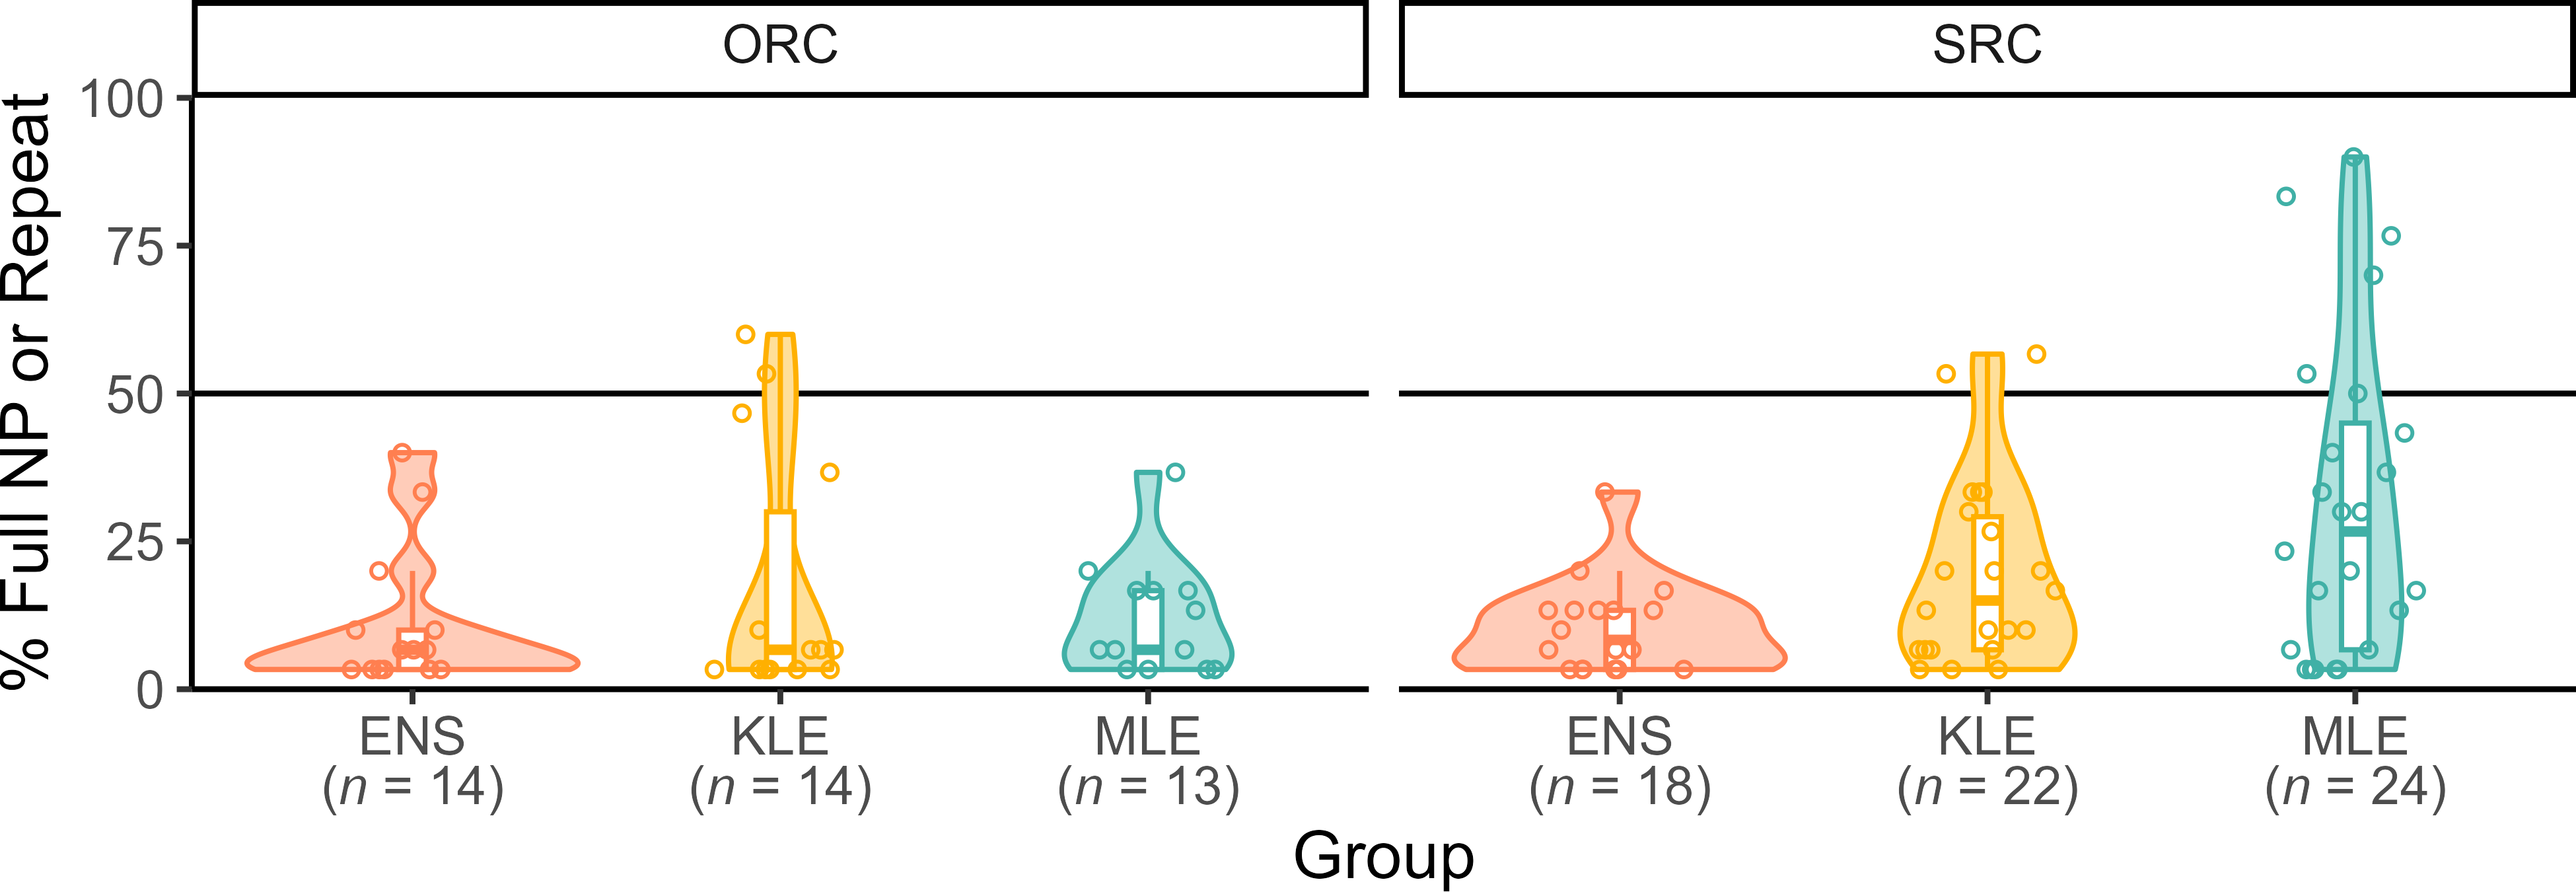
\includegraphics{../analysis/plots/quotative.png}
\vspace{-12pt}
\end{figure}

\noindent Most of these participants only rarely produced responses of the Full~NP and Repeat varieties. It is very unlikely that participants who gave such responses in less 50\% of trials thought that the task was asking them to regurgitate the test sentences. There were only nine participants in total---all of them L2ers---who produced Full~NP and Repeat responses more than half of the time: two KLEs in the ORC study, two KLEs in the SRC study, and five MLEs in the SRC study. 

To further inspect the data from these nine individuals, I calculated the rates at which they gave each type of potentially quotative response. The resulting counts and percentages are shown in Table~\ref{tab:quotative}.

\begin{table}
\caption{Participants with high rates of Full~NP and Repeat responses}\label{tab:quotative}
\raggedright\setstretch{1}
\begin{tblr}{colspec={lX[r]X[r]X[r]X[r]}}\toprule
Participant & Tokens Full~NP & Tokens Repeat & Percent Full~NP & Percent Repeat\\
\midrule
KLE\_ORC\_21 & 13 & 5 & 43.33 & 16.67\\
KLE\_ORC\_58 & 15 & 1 & 50.00 & 3.33\\
KLE\_SRC\_11 & 1 & 16 & 3.33 & 53.33\\
KLE\_SRC\_20 & 1 & 15 & 3.33 & 50.00\\
MLE\_SRC\_14 & 2 & 19 & 6.67 & 63.33\\
MLE\_SRC\_32 & 2 & 14 & 6.67 & 46.67\\
MLE\_SRC\_37 & 26 & 1 & 86.67 & 3.33\\
MLE\_SRC\_55 & 2 & 21 & 6.67 & 70.00\\
MLE\_SRC\_56 & 8 & 17 & 26.67 & 56.67\\
\bottomrule
\end{tblr}
\vspace{-12pt}
\end{table}

\noindent Five of these nine participants had only one or two Full~NP responses, suggesting that if they thought they were supposed to be repeating the test sentences, then they did not regard starting their response with \textit{The man/woman that}\dots{} as an important part of the procedure. 

Even if we remove all nine of the participants in Table~\ref{tab:quotative} from the data, though, there are still clear increases in each group's Resumption responses across conditions from Short to Long to Island (see~Appendix~\ref{app-results-ept}, Figures~\ref{fig:app-ept-token-orc-quotative} and \ref{fig:app-ept-token-src-quotative}). In fact, the same overall pattern of results is preserved even if Full~NP responses are recoded as Nontarget, leaving only instances of RP resumption in the Resumption category (see~Appendix~\ref{app-results-ept}, Figures~\ref{fig:app-ept-token-orc-quotative2} and \ref{fig:app-ept-token-src-quotative2}).

%========================================================%
\section{L2 proficiency effects for resumption rates}\label{ept-result-proficiency}
%========================================================%

Finally, we turn to RQ3, which asks how L2 proficiency affects rates of resumption. Recall that the L2 groups were closely aligned in terms of English proficiency, as explained in Section~\ref{stu-proficiency}.  Figures \ref{fig:ept-token-proficiency-orc} and \ref{fig:ept-token-proficiency-src} show the relationship between the scaled English proficiency scores and the mean response rates for L2ers in, respectively, the ORC data and the SRC data. Five participants had to be excluded from this analysis due to missing proficiency scores: in the ORC dataset, two KLEs and one MLE; in the SRC dataset, two MLEs.

\begin{figure}
\caption{Relationship between L2 proficiency and response rates in the ORC elicited production task} \label{fig:ept-token-proficiency-orc}
\raggedright\setstretch{1}
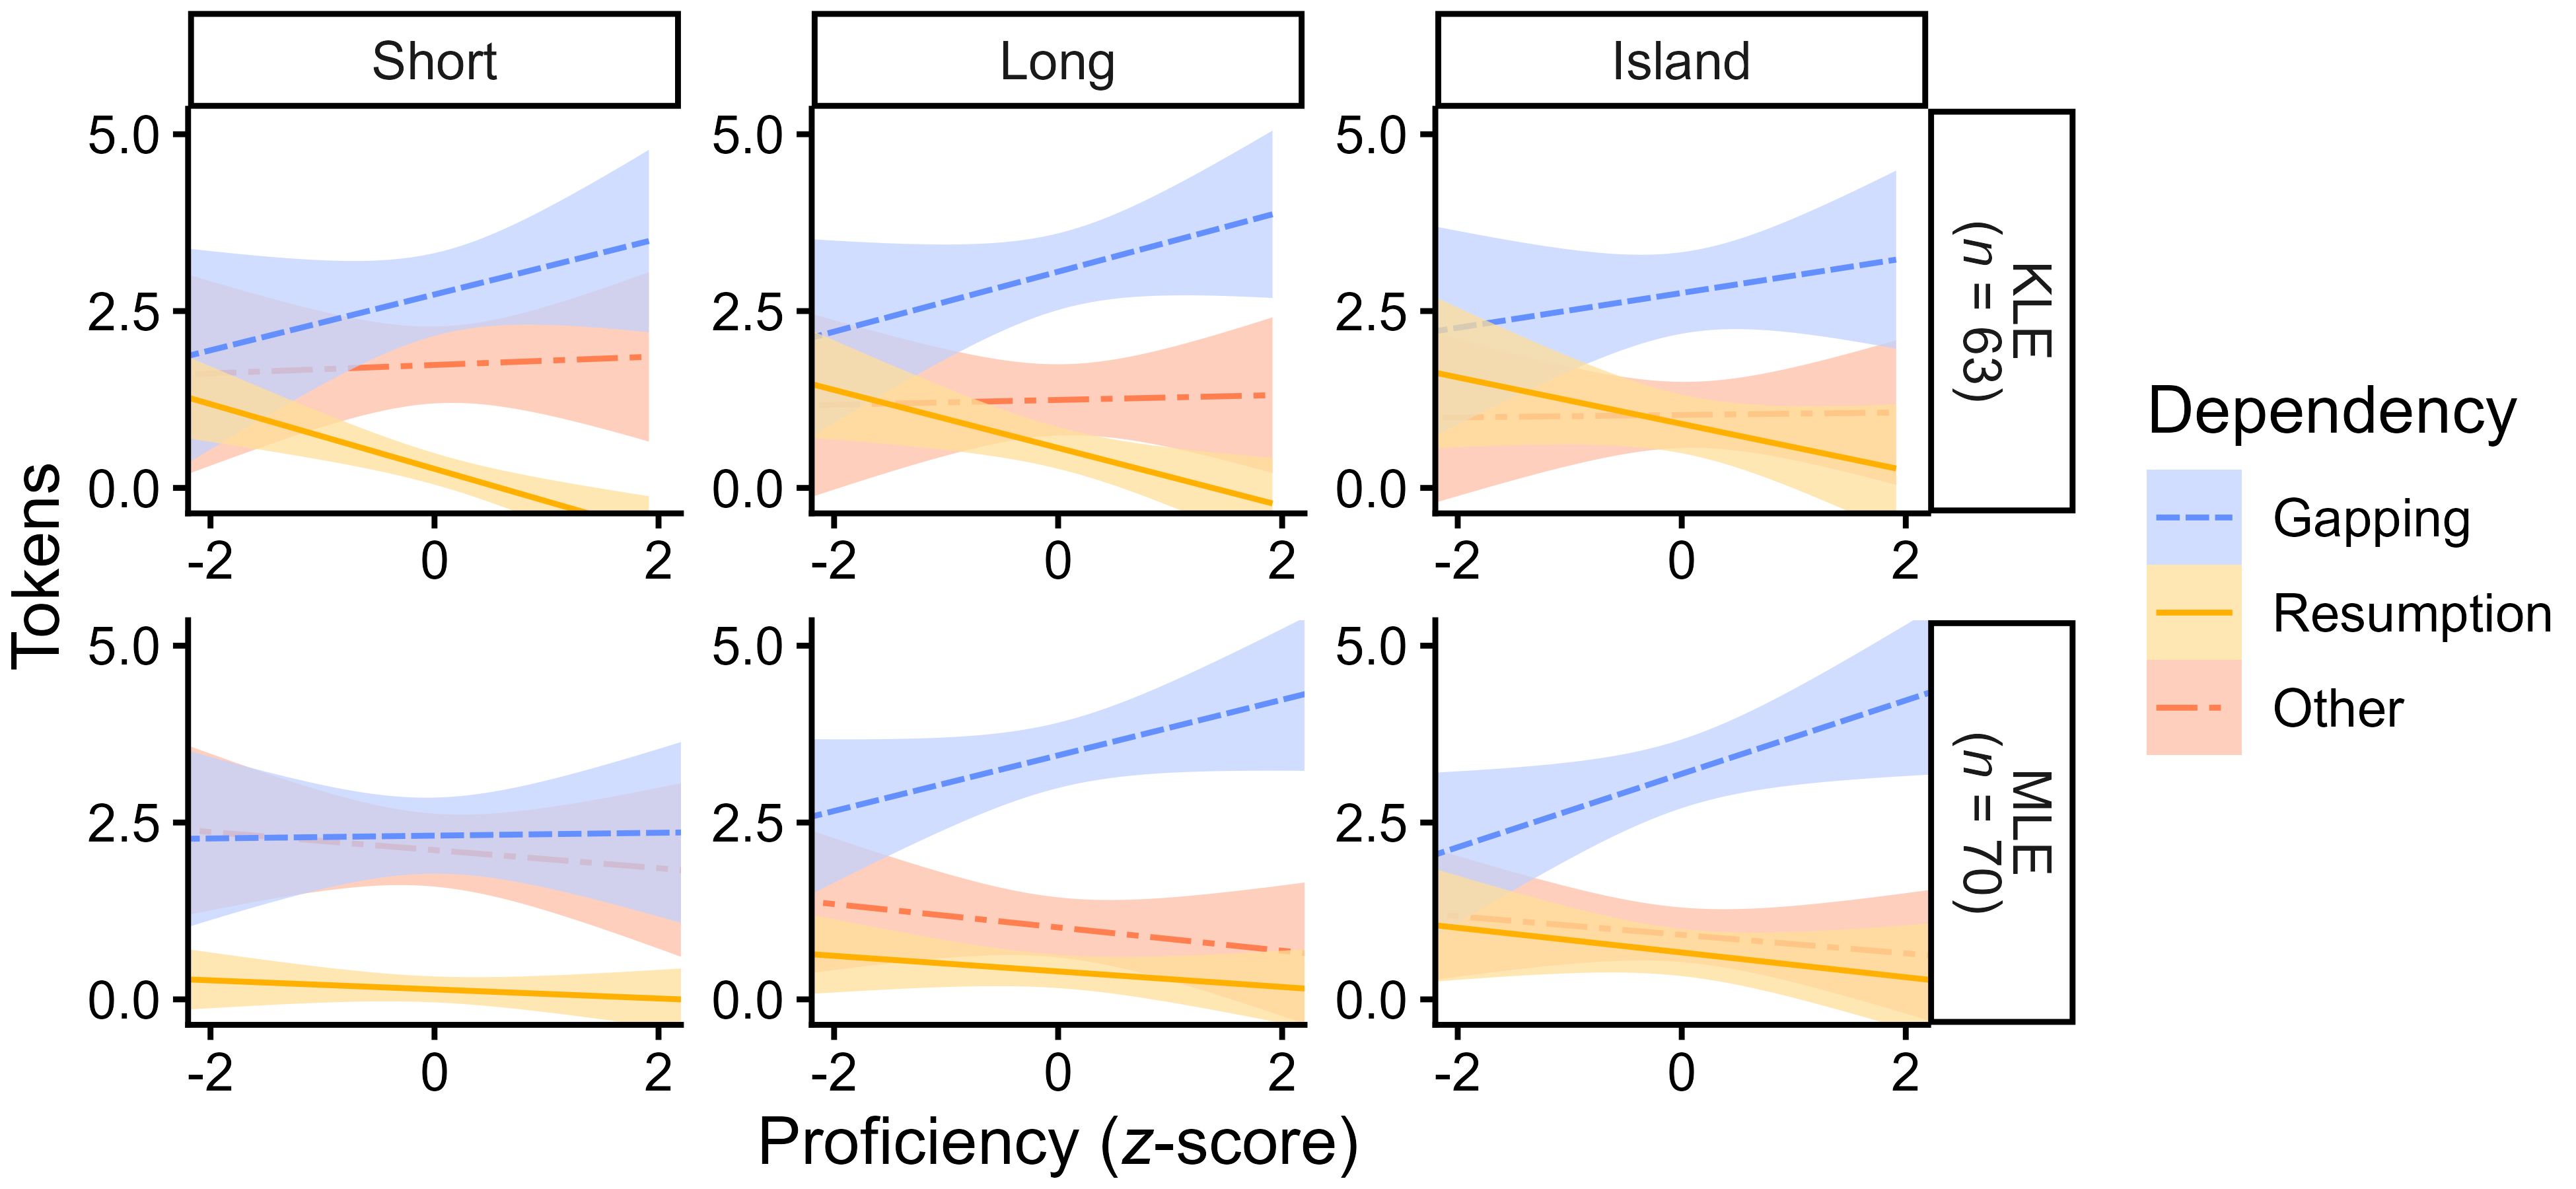
\includegraphics{../analysis/plots/orc_ept_token_proficiency.png}
\textit{Note}. Shading indicates 95\% \textit{CI}s.
\vspace{-12pt}
\end{figure}

\begin{figure}
\caption{Relationship between L2 proficiency and response rates in the SRC elicited production task} \label{fig:ept-token-proficiency-src}
\raggedright\setstretch{1}
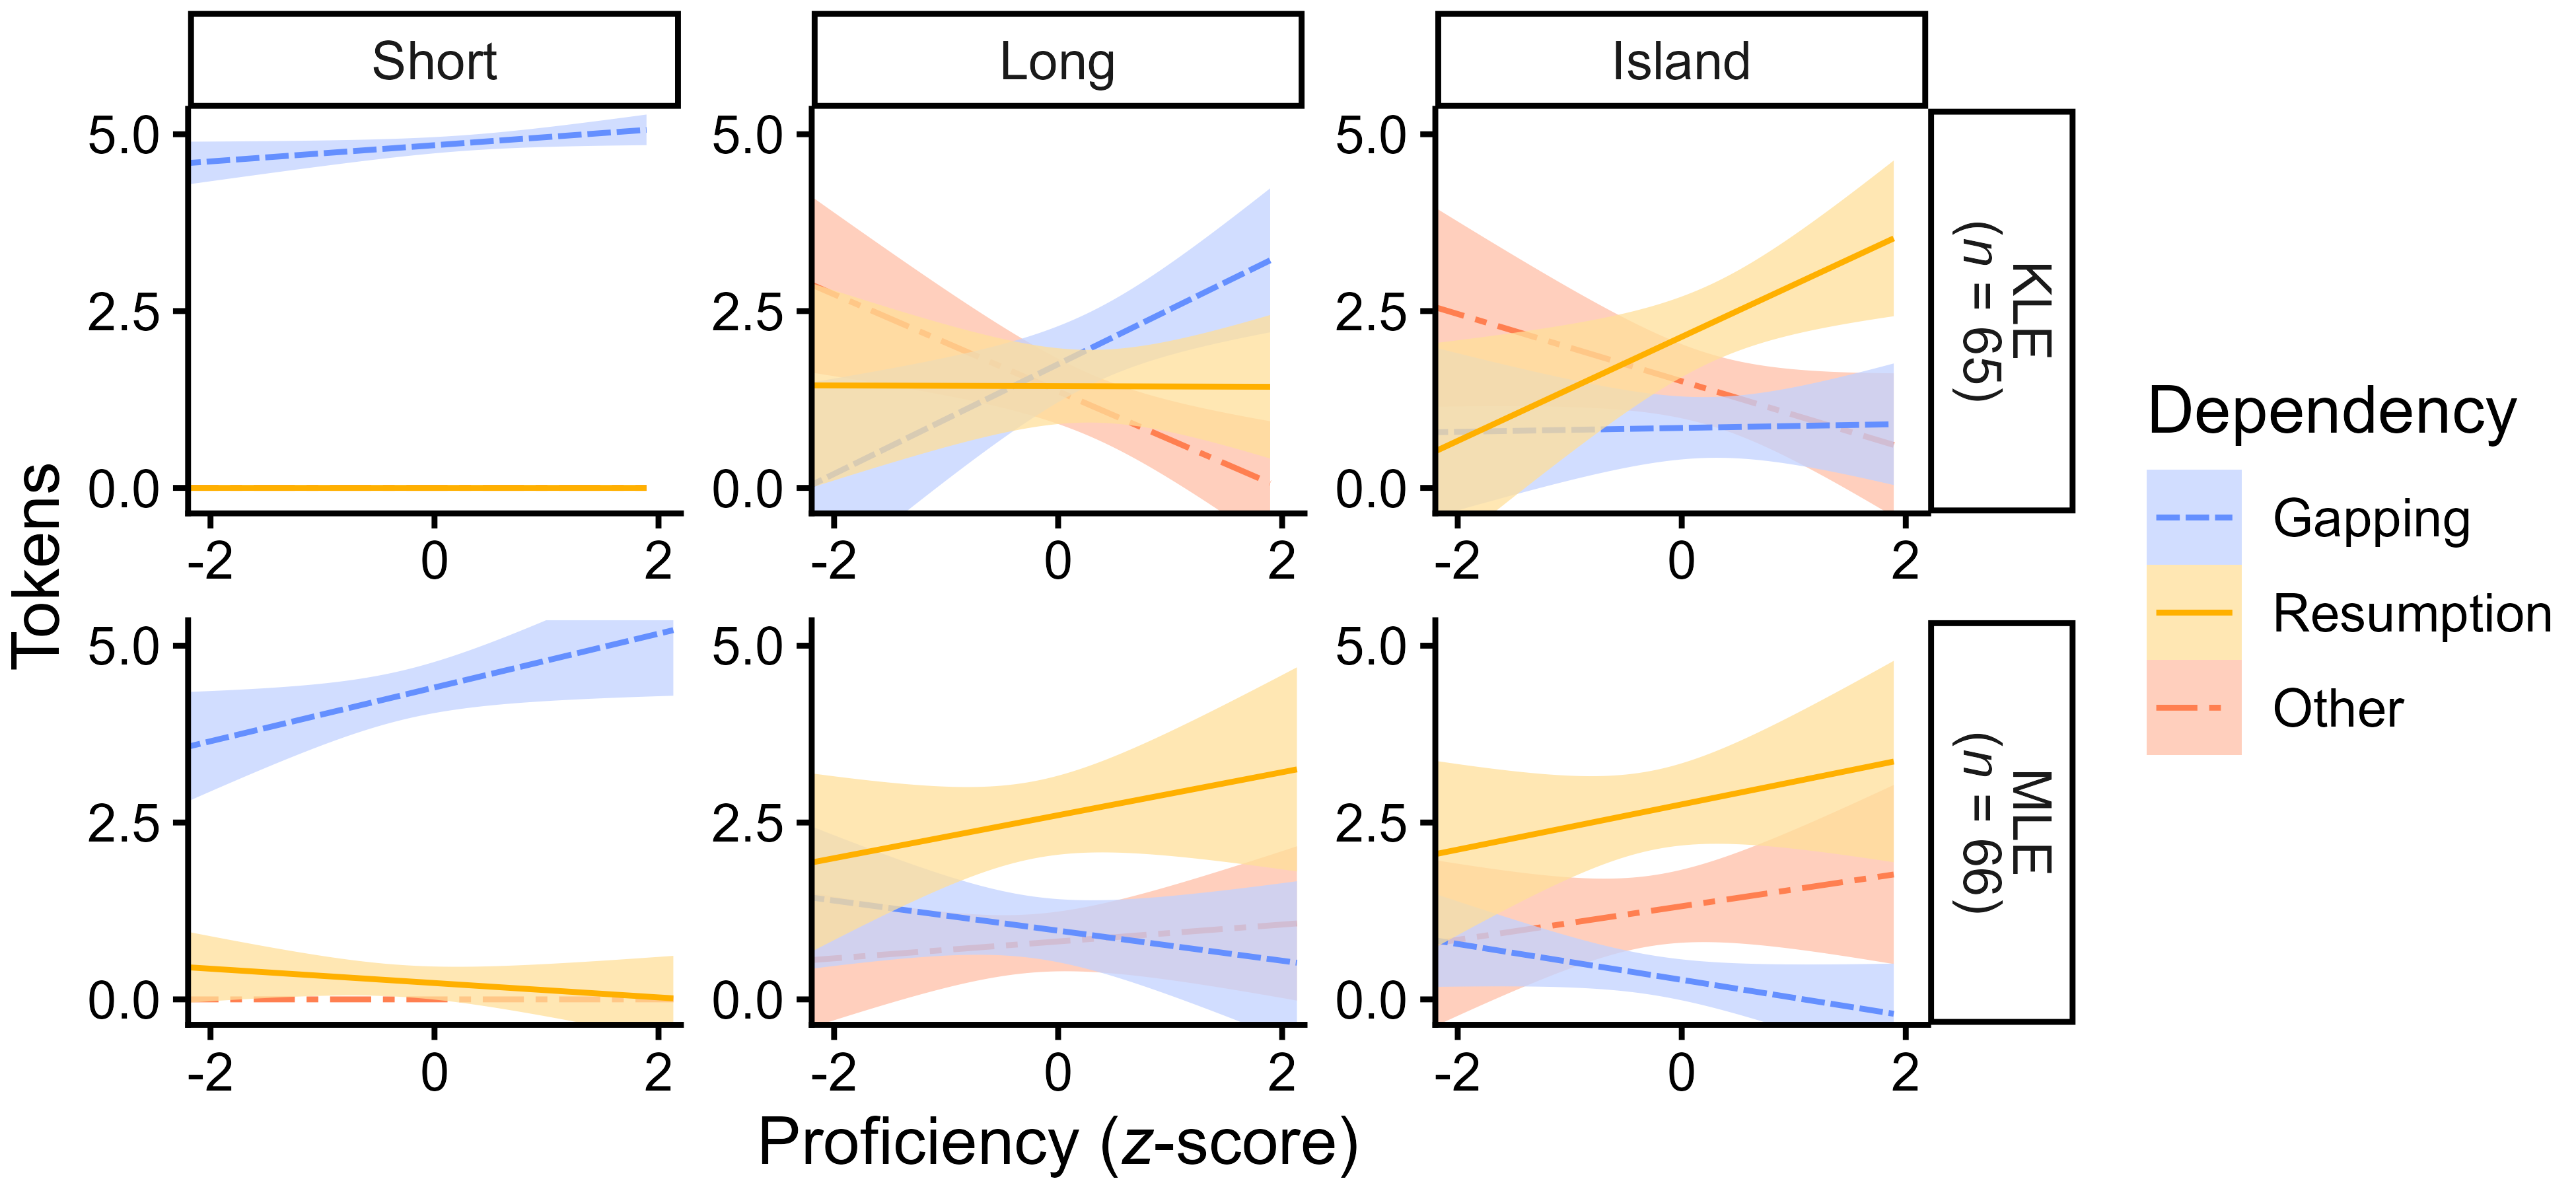
\includegraphics{../analysis/plots/src_ept_token_proficiency.png}
\textit{Note}. Shading indicates 95\% \textit{CI}s.
\vspace{-12pt}
\end{figure}

In the ORC data, there was an apparent \textsc{dependency × proficiency} interaction such that Gapping responses tended to increase with rising proficiency whereas Resumption responses tended to decrease with rising proficiency. This interaction seems to have been strongest in the case of KLE responses in the Short and Long conditions, though it could be seen to one degree or another in all the other combinations of \textsc{group} and \textsc{condition}.

The pattern of results was less uniform in the SRC data. The \textsc{dependency × proficiency} interaction here is only visible in the Short condition, but it is somewhat harder to spot because gapping rates are at or near ceiling and resumption rates are at or near floor, even for L2ers with relatively low proficiency scores. Elsewhere in the SRC plots, especially in the Island condition, we see an altogether different pattern such that as proficiency scores get higher, resumption rates tend to increase and gapping rates tend to decrease. This latter interaction appears to have been strongest for KLEs and MLEs in the Island condition, but it can also be seen in the Long condition for MLEs.

To further probe for L2 proficiency effects on resumption rates, I repeated the mixed-effects model analyses for the ORC and SRC datasets (separately) with \textsc{proficiency} added as a continuous fixed effect. 

The model for the ORC dataset (model formula: \textsc{resumption \~{} environment * group * proficiency + (1 + environment | participant) + (1 + environment + group | item)}---see~Appendix~\ref{app-results-ept}, Table~\ref{tab:app-orc-ept-resumption-proficiency-model} for details) yielded a significant effect for \textsc{proficiency} ($\hat{\beta}$~=~−1.71, \textit{SE}~= 0.73, $p$~= .019), indicating that Resumption responses decreased as proficiency scores went up. There was also a marginally significant effect for \textsc{environment} (Long − Short: $\hat{\beta}$~=~8.81, \textit{SE}~= 4.90, $p$~= .072) resulting from the fact that resumption rates were more common in the Long condition than in the Short condition, and a marginally significant \textsc{environment × proficiency} interaction ($\hat{\beta}$~=~2.79, \textit{SE}~= 1.66, $p$~= .093) suggesting that the strength of the proficiency effect differed more between the Long and Short conditions than it did between the Island and Short conditions. However, pairwise comparisons did not find the relationship between resumption rates and proficiency scores to be significant in any of the \textsc{environment × group} combinations when considered separately (all $p$s~>~.05).

The model for the SRC dataset (model formula: \textsc{resumption \~{} environment * group * proficiency + (1 + environment | participant) + (1 | item)}---see~Appendix~\ref{app-results-ept}, Table~\ref{tab:app-src-ept-resumption-proficiency-model} for details) found no significant effects for \textsc{proficiency} or for the interactions between \textsc{proficiency} and the other factors in the analysis. Pairwise comparisons revealed that the proficiency effect approached significance only for the KLE data in the Island environment, where higher proficiency scores were associated with higher resumption rates ($\hat{\beta}$~=~2.13, \textit{SE}~= 0.86, $p$~= .072).

To review, these results broadly indicate that L2ers tend to produce resumptive RCs less often as their proficiency level rises, at least in syntactic environments where English only permits gapping. The effect is strongest in the ORC Short and ORC Long conditions, and its weakness in the SRC Short condition can be explained by the fact that resumption responses were at or near floor in that environment across the proficiency spectrum. That resumption rates actually increase in the SRC Island condition is not anomalous given that (a)~English prohibits gaps in that environment and (b)~ENSs also resort to resumption at high rates there; producing more resumptive RCs in the SRC Island condition therefore brings L2ers more in line with native-speaker performance.

%========================================================%
\section{Summing up}\label{ept-conclusion}
%========================================================%

This chapter reported the ORC and SRC results from the EPT. The data analyses revealed that all groups produced resumptive RCs more often in environments thought to be relatively difficult for relativization than in environments thought to be relatively easy for relativization. Whereas ENSs and MLEs both displayed a strong preference for RP resumption over full-NP resumption, KLEs did not display nearly as strong a preference for one form of resumption over the other. Finally, proficiency effects were observed in the L2 data such that resumption rates declined in the ORC dataset with rising proficiency, especially in the Short and Long conditions (where English requires gapping), while the opposite pattern was observed in the SRC dataset, at~least in the Island environment (where English lacks grammatical relativization and ENSs also produce resumptive RCs at high rates). Overall, the combination of these patterns of results is consistent with the idea of resumption easing the production of RCs under processing strain.